Os pilares podem estar submetidos à forças normais e momentos fletores, gerando compressão simples e flexão composta.

\begin{itemize}

	\item \textbf{Compressão simples}: Também chamada de compressão centrada ou compresão uniforme, é caracterizada pela aplicação da força normal $(N_d)$ no centro geométrico da seção transversal do pilar.

		\begin{figure}[H]
			\begin{center}
				\caption{Solicitação normal acontecendo no centro geométrico da seção transversal do pilar.}    	
				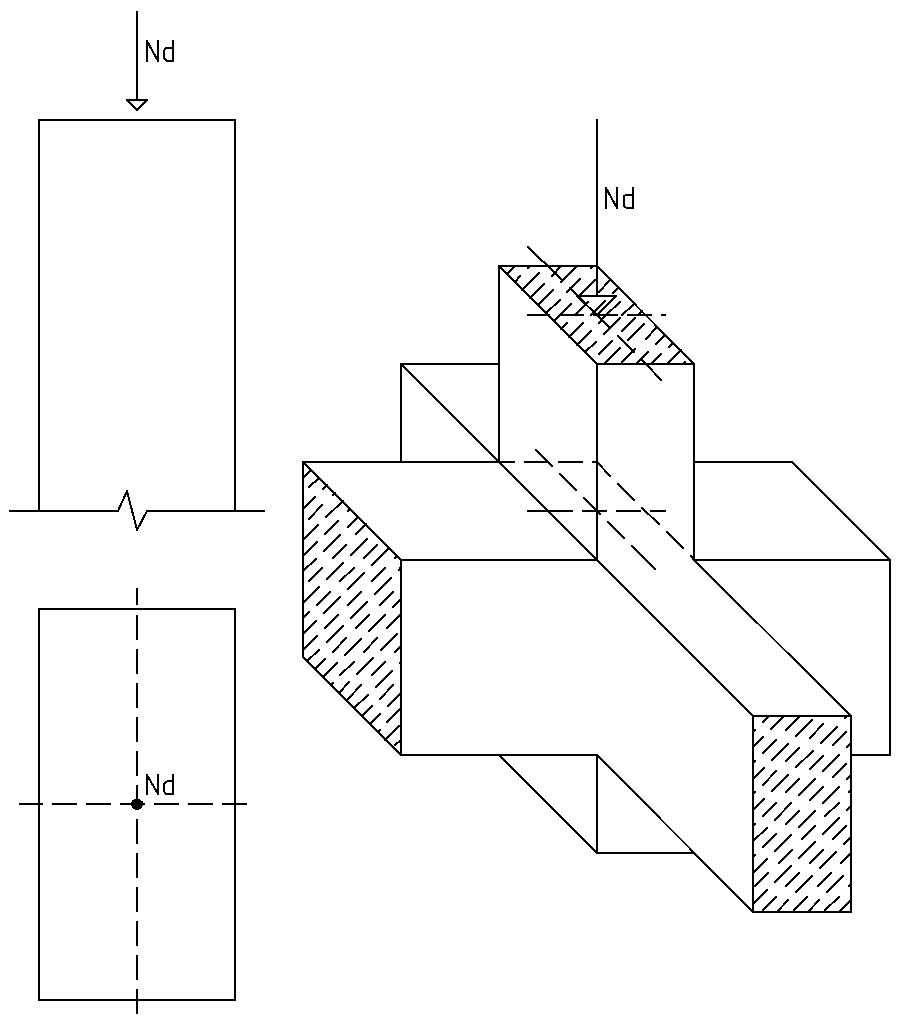
\includegraphics[height=0.5\textwidth]{Solicitacoes-normais/Imagens/Compressao-simples.png}
			\end{center}
		\end{figure}

	\item \textbf{Flexão composta}: Ocorre força normal e momento fletor sobre o pilar. Há dois casos:

		\begin{itemize}
     			\item \textit{Flexão composta normal (ou reta)}: Existe a força normal e um momento fletor em uma direção, sendo:
				$$M1_{dx}=e1_x\cdot N_d$$

				\begin{figure}[H]
					\begin{center}
						\caption{Solicitação normal acontecendo fora do centro geométrico da seção transversal do pilar, em apenas uma direção.}    	
						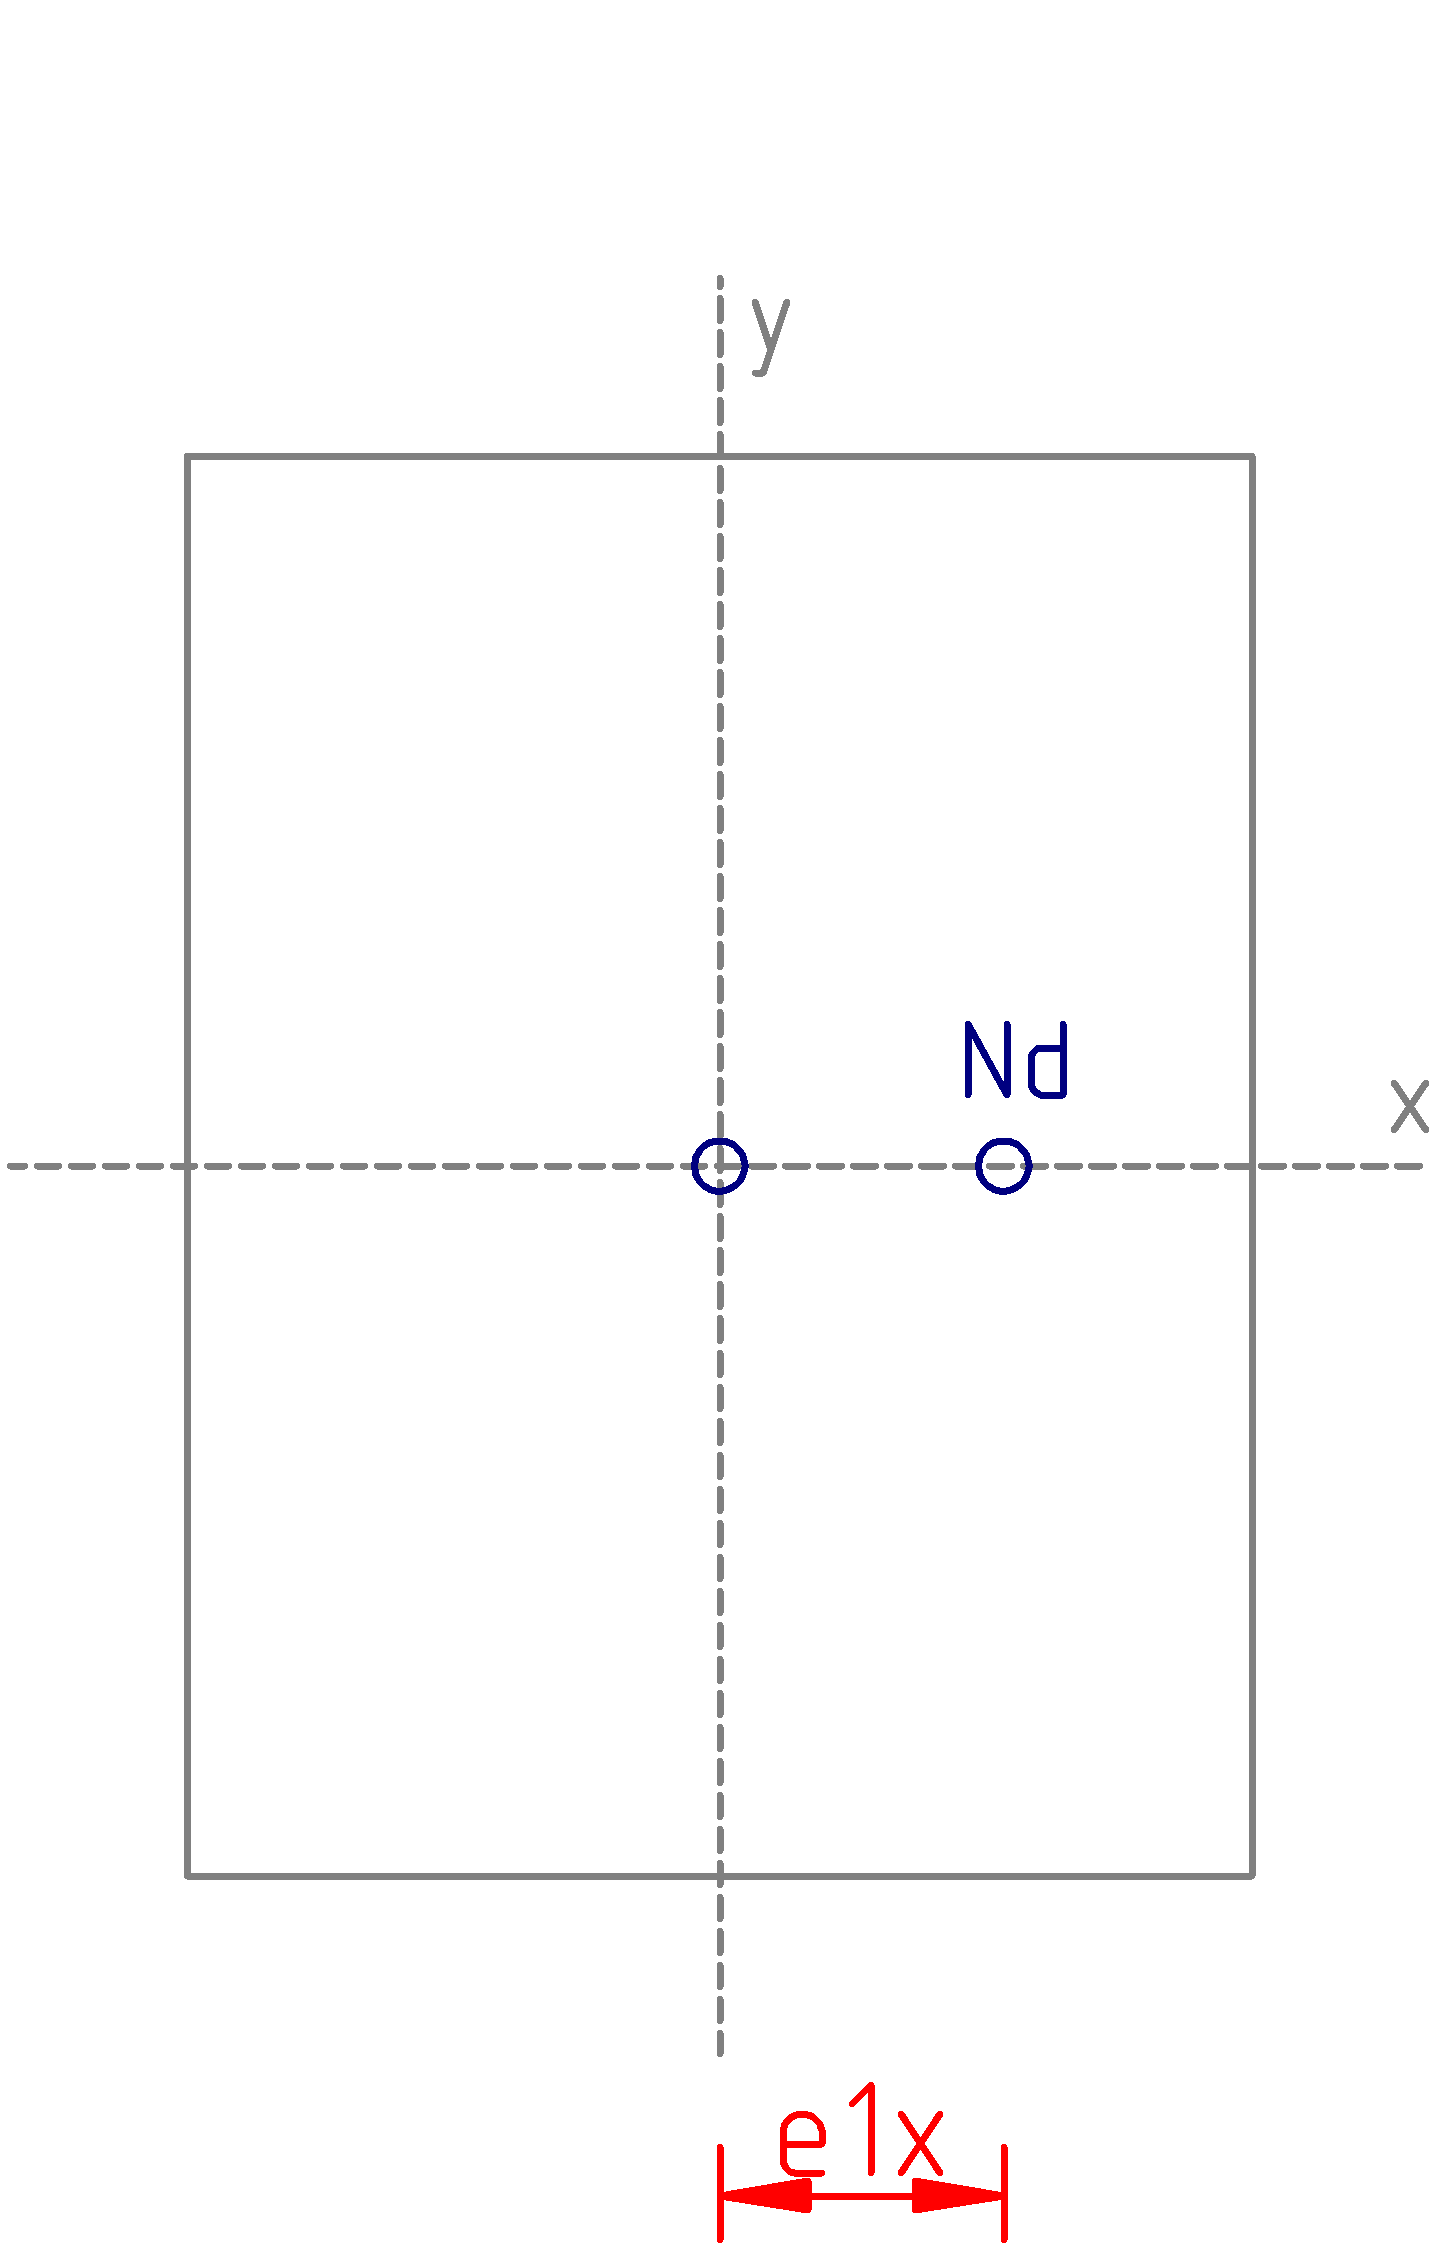
\includegraphics[height=0.4\textwidth]{Solicitacoes-normais/Imagens/Flexao-composta-normal.png}
					\end{center}
				\end{figure}
				
     			\item \textit{Flexão composta oblíqua}: Existe força normal e dois momentos fletores, sendo:
				$$M1_{dx}=e1_x\cdot N_d$$
				$$M1_{dy}=e1_y\cdot N_d$$

				\begin{figure}[H]
					\begin{center}
						\caption{Solicitação normal acontecendo fora do centro geométrico da seção transversal do pilar, em duas direções.}    	
						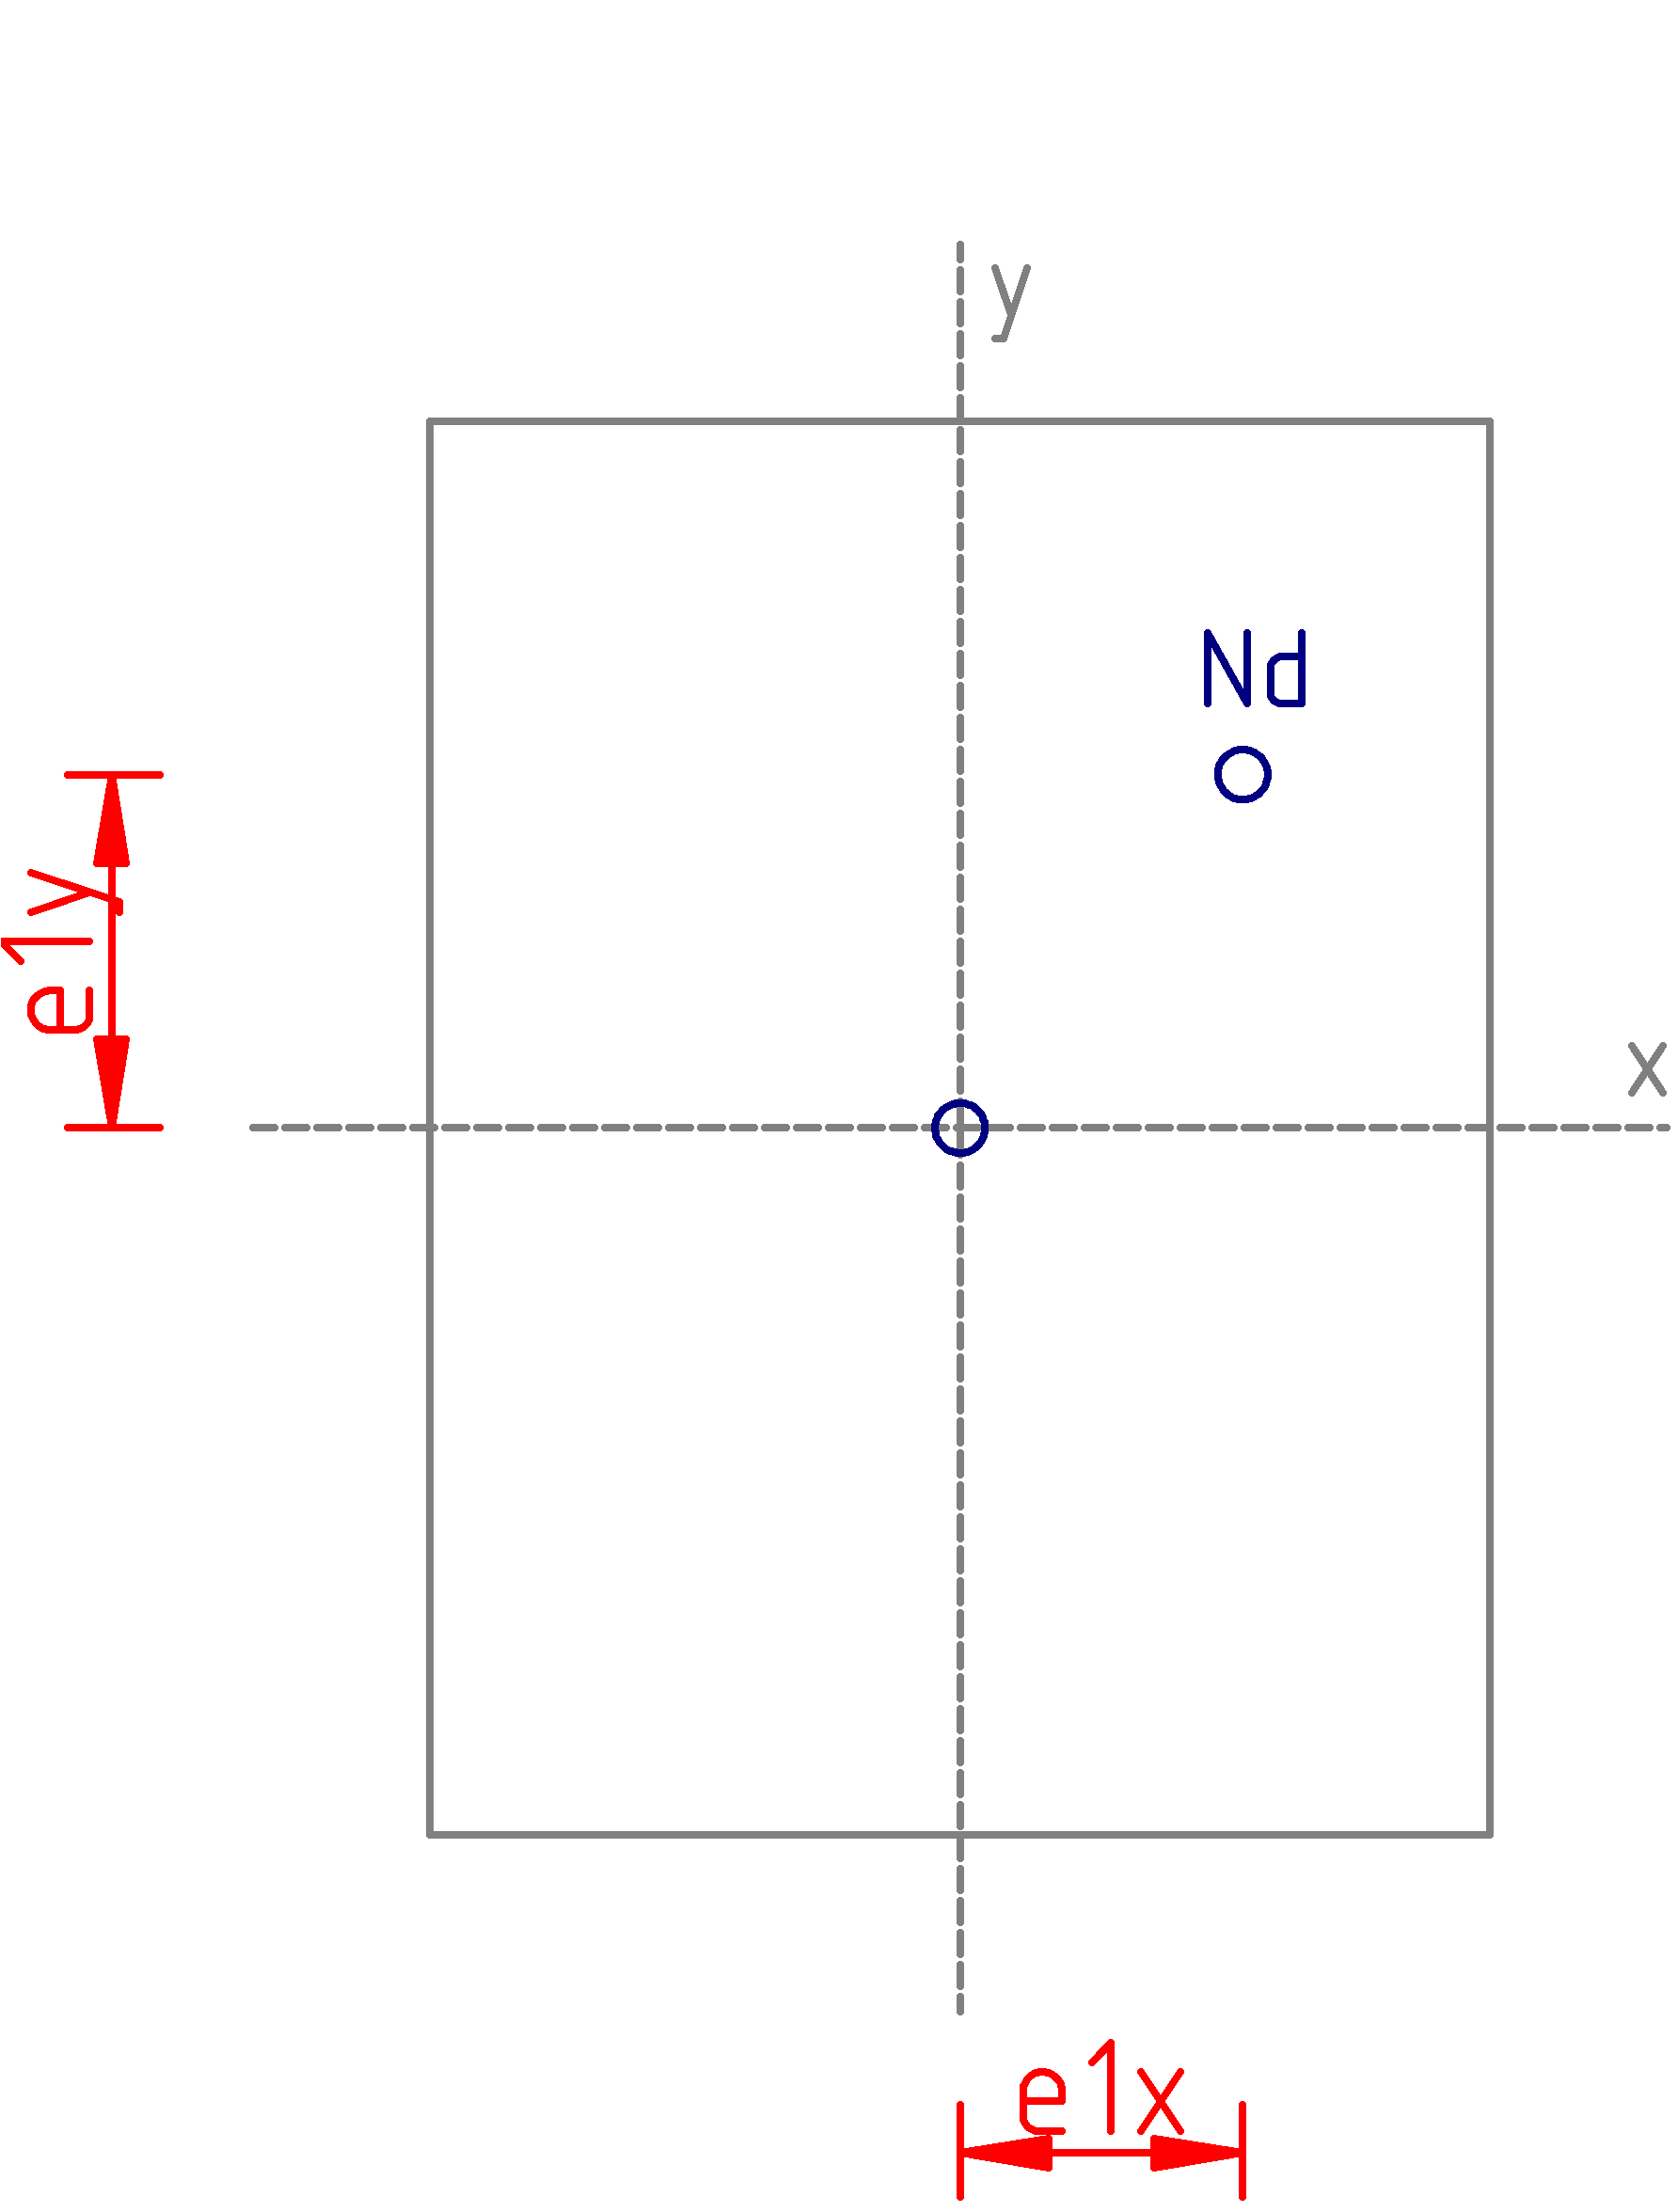
\includegraphics[height=0.45\textwidth]{Solicitacoes-normais/Imagens/Flexao-composta-obliqua.png}
					\end{center}
				\end{figure}

  		\end{itemize}

\end{itemize}

